\section{曲线积分：基本概念及性质}
\entry{定义 5.2.1}{第一型曲线积分}{p.258}
设 $L$ 为 $\mathbb R^3$ 中可求长曲线，端点为 $A,B$。依次取分点
\[
A=A_0,A_1,\ldots,A_n=B,
\]
构成分割 $T$；弧段 $L_i=A_{i-1}A_i$ 的弧长记为 $\Delta s_i$，分割细度为 $\lambda=\max_i\Delta s_i$。在 $L_i$ 上任取 $P_i=(\xi_i,\eta_i,\zeta_i)$，令
\[
S(f,T)=\sum_{i=1}^n f(P_i)\Delta s_i.
\]
若存在 $I$，使任意 $\varepsilon>0$，存在 $\delta>0$，只要 $\lambda<\delta$，不论介点如何选择，均有 $|S(f,T)-I|<\varepsilon$，则称 $f$ 在 $L$ 上可积，记为
\[
I=\int_L f(x,y,z)\dd s=\int_L f\dd s.
\]
\begin{center}\begin{minipage}{\linewidth}\centering
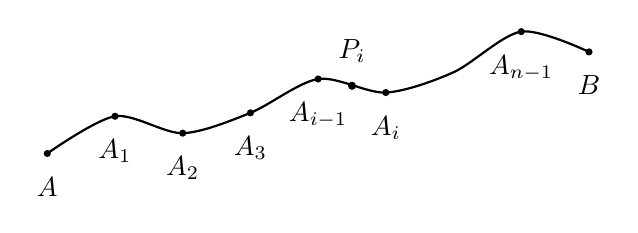
\begin{tikzpicture}[scale=.86]
\draw[thick] plot[smooth] coordinates {(0,0)(1,.55)(2,.3)(3,.6)(4,1.1)(5,.9)(6,1.2)(7,1.8)(8,1.5)};
\foreach \x/\y/\lab in {0/0/A,1/.55/A_1,2/.3/A_2,3/.6/A_3,4/1.1/A_{i-1},5/.9/A_i,7/1.8/A_{n-1},8/1.5/B}{\fill (\x,\y) circle(1.5pt) node[below=5pt] {$\lab$};}
\fill (4.5,1) circle(1.7pt) node[above=5pt] {$P_i$};
\end{tikzpicture}
\par{\small 图 5.2.1\quad 曲线分割示意（重绘）}
\end{minipage}\end{center}

\entry{定义 5.2.2}{第二型曲线积分}{p.259}
设 $\FF=(P,Q,R)$ 为空间区域 $D$ 中的向量场，$L\subset D$ 为从 $A$ 到 $B$ 的可求长有向曲线。顺序取分点 $\rr_0=A,\ldots,\rr_n=B$，记
\[
\Delta\rr_i=\rr_i-\rr_{i-1},\qquad \|T\|=\max_i|\Delta\rr_i|.
\]
在各弧段上任取 $\vct\xi_i$，若极限
\[
\lim_{\|T\|\to0}\sum_{i=1}^n\FF(\vct\xi_i)\cdot\Delta\rr_i
\]
为定数，则记为 $\int_L\FF\cdot\dd\rr$。闭曲线 $L$ 上的积分称为环量，记为 $\oint_L\FF\cdot\dd\rr$。因 $\rr=(x,y,z)$、$\dd\rr=(\dd x,\dd y,\dd z)$，也记为
\[
\int_L\FF\cdot\dd\rr=\int_L P\dd x+Q\dd y+R\dd z.
\]

\entry{定理 5.2.1}{第一型曲线积分的参数计算}{p.259}
设 $L\subset\mathbb R^3$ 为光滑曲线，其参数为
$\vct\varphi(t)=(x(t),y(t),z(t))$，$\alpha\le t\le\beta$，且 $f$ 在 $L$ 上连续，则
\[
\int_L f\dd s=\int_\alpha^\beta(f\circ\vct\varphi)(t)|\vct\varphi'(t)|\dd t.
\]
\textbf{注 5.2.1}\quad 此公式将第一型曲线积分化为区间上的 Riemann 积分。

\entry{定理 5.2.2}{第二型曲线积分的参数计算}{pp.259—260}
设 $D\subset\mathbb R^3$ 为区域，$\FF:D\to\mathbb R^3$ 连续，$L\subset D$ 为有向光滑曲线，参数 $\rr=\rr(t)$，$\alpha\le t\le\beta$，参数增加方向与 $L$ 一致，则
\[
\int_L\FF\cdot\dd\rr=\int_\alpha^\beta(\FF\circ\rr)(t)\cdot\rr'(t)\dd t.
\]
当 $\FF=(P,Q,R)$ 时，右端为
\[
\int_\alpha^\beta\bigl[P(\rr(t))x'(t)+Q(\rr(t))y'(t)+R(\rr(t))z'(t)\bigr]\dd t.
\]
\textbf{注 5.2.2}\quad 此公式将第二型曲线积分化为区间上的 Riemann 积分。

\entry{性质}{第二型曲线积分的基本性质}{p.260}
\textbf{（1）线性。} 若 $\FF=c_1\FF_1+c_2\FF_2$，则
\[
\int_L\FF\cdot\dd\rr=c_1\int_L\FF_1\cdot\dd\rr+c_2\int_L\FF_2\cdot\dd\rr.
\]
特别地，对 $\FF_1=P\vct i$、$\FF_2=Q\vct j$、$\FF_3=R\vct k$，有
\[
\int_L\FF\cdot\dd\rr=\int_L P\dd x+Q\dd y+R\dd z
=\int_L P\dd x+\int_L Q\dd y+\int_L R\dd z.
\]
\textbf{（2）路径可加性。} 若 $L_{AC}$ 由 $L_{AB}$ 与 $L_{BC}$ 连接而成，则
\[
\int_{L_{AC}}\FF\cdot\dd\rr=\int_{L_{AB}}\FF\cdot\dd\rr+\int_{L_{BC}}\FF\cdot\dd\rr.
\]
因此，逐段光滑曲线可以分段积分。

\textbf{（3）方向性。}
\[
\int_{L_{AB}}\FF\cdot\dd\rr=-\int_{L_{BA}}\FF\cdot\dd\rr.
\]

\entry{定理 5.2.3}{Green 公式}{p.260}
设 $D$ 为有限条逐段光滑封闭曲线 $L$ 围成的平面闭区域，$\FF=(P(x,y),Q(x,y))$ 为 $D$ 上光滑场，则
\[
\oint_L P\dd x+Q\dd y=\iint_D\left(\frac{\partial Q}{\partial x}-\frac{\partial P}{\partial y}\right)\dd x\dd y,
\]
其中 $L=\partial D$ 取行进时 $D$ 在左侧的方向。

\entry{定义 5.2.3}{有势场与势函数}{p.260}
设 $\FF=(P,Q,R)$ 定义于 $V\subset\mathbb R^3$。若存在数量场 $\varphi$，使
\[
\grad\varphi(\vct p)=\FF(\vct p),\qquad\forall\vct p\in V,
\]
则称 $\FF$ 有势，$\varphi$ 为势函数，即 $\varphi_x=P$、$\varphi_y=Q$、$\varphi_z=R$。

\entry{定义 5.2.4}{保守场}{p.260}
若 $\FF$ 对 $V$ 内任意有向闭路 $L$ 均有 $\oint_L\FF\cdot\dd\rr=0$，则称 $\FF$ 为保守场。

\entry{定理 5.2.4}{保守与有势}{p.261}
向量场保守的充要条件为有势。

\entry{定理 5.2.5}{无旋与有势的判据}{p.261}
在曲面单连通的区域 $V$ 上，光滑向量场 $\FF$ 是有势场的充要条件是它是无旋场，即在 $V$ 中每点 $\rot(\FF)$ 是零向量。
\ednote{原书作“曲面单连通”；此处有势判据通常要求路径（线）单连通，使用时应核对区域假设。}

\clearpage
\section{曲线积分：例题及原解}
\entry{例 5.2.1}{圆周上的第一型积分}{p.261}
求 $I=\int_L\sqrt{x^2+y^2}\dd s$，其中 $L:x^2+y^2=ax$，$a>0$。
\sol 取参数
\[
x=\frac a2+\frac a2\cos t,\quad y=\frac a2\sin t,\quad 0\le t\le2\pi.
\]
则 $\rr'(t)=(-\frac a2\sin t,\frac a2\cos t)$，$\dd s=\frac a2\dd t$。于是
\[
I=\frac{a^2}{2}\int_0^{2\pi}\left|\cos\frac t2\right|\dd t
=a^2\int_0^\pi|\cos t|\dd t=2a^2.
\]
\ednote{原书首个代入式根号内疑多一因子 $a$；此处按所列参数式与后续等式整理，仅保留原解后续正确计算链。}

\entry{例 5.2.2}{第一象限椭圆弧}{p.261}
设 $L$ 为 $x^2/a^2+y^2/b^2=1$（$a,b>0$）在第一象限的弧，求 $\int_Lxy\dd s$。
\sol 令 $x=a\cos\theta$，$y=b\sin\theta$，$0\le\theta\le\pi/2$，则
\begin{align*}
I&=ab\int_0^{\pi/2}\cos\theta\sin\theta\sqrt{a^2\sin^2\theta+b^2\cos^2\theta}\dd\theta\\
&=\frac{ab}{2}\int_0^{\pi/2}\sqrt{b^2+(a^2-b^2)\sin^2\theta}\dd(\sin^2\theta)\\
&=\frac{ab}{2}\int_0^1\sqrt{b^2+(a^2-b^2)t}\dd t
=\frac{ab(a^2+ab+b^2)}{3(a+b)}.
\end{align*}

\entry{例 5.2.3}{三角形边界上的弧长积分}{pp.261—262}
求 $\int_Lx\dd s$，其中 $L$ 为 $O(0,0)$、$A(1,0)$、$B(0,1)$ 所成三角形的边界。
\sol 将曲线分段，均取 $0\le t\le1$：
\[
\begin{array}{c|ccc}
 &x&y&\dd s\\\hline
OA&t&0&\dd t\\
AB&1-t&t&\sqrt2\dd t\\
BO&0&1-t&\dd t
\end{array}
\]
因此
\begin{align*}
I&=\int_{OA}x\dd s+\int_{AB}x\dd s+\int_{BO}x\dd s\\
&=\int_0^1t\dd t+\int_0^1(1-t)\sqrt2\dd t+\int_0^10\dd t
=\frac{1+\sqrt2}{2}.
\end{align*}
\begin{center}\begin{minipage}{\linewidth}\centering
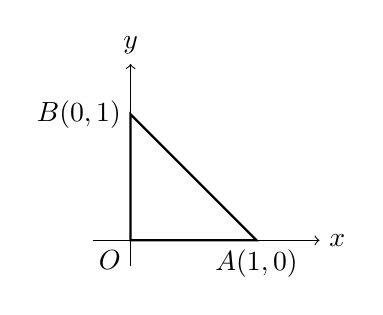
\begin{tikzpicture}[scale=1.6]
\draw[->](-.3,0)--(1.5,0)node[right]{$x$};\draw[->](0,-.2)--(0,1.4)node[above]{$y$};
\draw[thick](0,0)--(1,0)--(0,1)--cycle;
\node[below left]at(0,0){$O$};\node[below]at(1,0){$A(1,0)$};\node[left]at(0,1){$B(0,1)$};
\end{tikzpicture}\par{\small 图 5.2.2\quad 三角形边界（重绘）}
\end{minipage}\end{center}

\entry{例 5.2.4}{球面与平面交圆的对称性}{p.262}
求 $I=\int_Lxy\dd s$，其中 $L$ 为球面 $x^2+y^2+z^2=a^2$ 与平面 $x+y+z=0$ 的交圆。
\sol 由对称性，$\int_Lxy\dd s=\int_Lyz\dd s=\int_Lzx\dd s$。因此
\begin{align*}
I&=\frac13\int_L(xy+yz+zx)\dd s\\
&=\frac16\int_L\bigl[(x+y+z)^2-(x^2+y^2+z^2)\bigr]\dd s\\
&=-\frac16\int_La^2\dd s=-\frac16a^2\cdot2\pi a=-\frac{\pi a^3}{3}.
\end{align*}

\entry{例 5.2.5}{锥面与柱面交线上的积分}{pp.262—263}
求 $I=\int_Lz\dd s$，其中 $L$ 为 $x^2+y^2=z^2$ 和 $y^2=ax$（$a>0$）的交线从 $(0,0,0)$ 到 $(a,a,a\sqrt2)$ 的弧。
\sol 取 $y=t$，则
\[
\rr(t)=\left(\frac{t^2}{a},t,\frac{t\sqrt{t^2+a^2}}{a}\right),\quad 0\le t\le a,
\qquad |\rr'(t)|=\frac1a\sqrt{\frac{8t^4+9a^2t^2+2a^4}{t^2+a^2}}.
\]
于是
\begin{align*}
I&=\int_0^a\frac{t\sqrt{t^2+a^2}}a\cdot\frac1a\sqrt{\frac{8t^4+9a^2t^2+2a^4}{t^2+a^2}}\dd t\\
&=\frac1{a^2}\int_0^at\sqrt{8t^4+9a^2t^2+2a^4}\dd t\\
&=\frac1{2a^2}\int_0^{a^2}\sqrt{8t^2+9a^2t+2a^4}\dd t\\
&=\frac{\sqrt2}{a^2}\int_0^{a^2}\sqrt{\left(t+\frac{9a^2}{16}\right)^2-\left(\frac{\sqrt{17}a^2}{16}\right)^2}\dd t.
\end{align*}
令 $u=t+9a^2/16$，$b=\sqrt{17}a^2/16$，则
\begin{align*}
I&=\frac{\sqrt2}{a^2}\int_{9a^2/16}^{25a^2/16}\sqrt{u^2-b^2}\dd u\\
&=\frac{17\sqrt2a^2}{256}\int_{9/\sqrt{17}}^{25/\sqrt{17}}\sqrt{t^2-1}\dd t\\
&=\frac{\sqrt2a^2}{512}\left[100\sqrt{38}-72-17\arcosh\frac{25}{\sqrt{17}}+17\arcosh\frac9{\sqrt{17}}\right].
\end{align*}

\entry{例 5.2.6}{三角形正向周界的第二型积分}{p.263}
求 $I=\oint_Lxy\dd x+x^2\dd y$，其中 $L$ 为 $O(0,0)$、$A(1,2)$、$B(0,2)$ 所成三角形的正向周界。
\sol 分为 $L_1=OA$、$L_2=AB$、$L_3=BO$，有
\begin{align*}
\int_{L_1}xy\dd x+x^2\dd y&=\int_0^1(x\cdot2x+2x^2)\dd x=4\int_0^1x^2\dd x=\frac43,\\
\int_{L_2}xy\dd x+x^2\dd y&=-2\int_0^1(1-x)\dd x=-1,\\
\int_{L_3}xy\dd x+x^2\dd y&=0.
\end{align*}
故 $I=4/3-1=1/3$。
\begin{center}\begin{minipage}{\linewidth}\centering
\begin{tikzpicture}[scale=1.1,midarrow/.style={postaction={decorate},decoration={markings,mark=at position .55 with {\arrow{Stealth}}}}]
\draw[->](-.3,0)--(1.8,0)node[right]{$x$};\draw[->](0,-.3)--(0,2.6)node[above]{$y$};
\draw[thick,midarrow](0,0)--(1,2);\draw[thick,midarrow](1,2)--(0,2);\draw[thick,midarrow](0,2)--(0,0);
\node[below left]at(0,0){$O$};\node[right]at(1,2){$A(1,2)$};\node[left]at(0,2){$B(0,2)$};
\end{tikzpicture}\par{\small 图 5.2.3\quad 有向三角形（重绘）}
\end{minipage}\end{center}

\entry{例 5.2.7}{球面与过轴平面的有向交圆}{pp.263—264}
求
\[
I=\oint_L(y-z)\dd x+(z-x)\dd y+(x-y)\dd z,
\]
其中 $L$ 为球面 $x^2+y^2+z^2=R^2$ 与平面 $y=x\tan\alpha$ 的交圆，从 $x$ 轴正向看去为顺时针，$0<\alpha<\pi/2$。
\sol 球面的参数为
\[
x=R\sin\theta\cos\varphi,\quad y=R\sin\theta\sin\varphi,\quad z=R\cos\theta,
\quad 0\le\theta\le\pi,\quad0\le\varphi\le2\pi.
\]
因 $L$ 又在平面上，故 $\tan\varphi=\tan\alpha$，即 $\varphi=\alpha$ 或 $\pi+\alpha$。两半圆为
\[
\begin{aligned}
L_1:\ &x=R\sin\theta\cos\alpha,\quad y=R\sin\theta\sin\alpha,\quad z=R\cos\theta,\\
L_2:\ &x=-R\sin\theta\cos\alpha,\quad y=-R\sin\theta\sin\alpha,\quad z=-R\cos\theta,
\end{aligned}\qquad 0\le\theta\le\pi.
\]
于是可以统一写为 $x=R\sin\theta\cos\alpha$、$y=R\sin\theta\sin\alpha$、$z=R\cos\theta$，$0\le\theta\le2\pi$。代入得
\begin{align*}
I=\int_0^{2\pi}\bigl[&(R\sin\theta\sin\alpha-R\cos\theta)(R\cos\theta\cos\alpha)\\
&+(R\cos\theta-R\sin\theta\cos\alpha)(R\cos\theta\sin\alpha)\\
&+(R\sin\theta\cos\alpha-R\sin\theta\sin\alpha)(-R\sin\theta)\bigr]\dd\theta\\
=R^2\int_0^{2\pi}&(\sin\alpha-\cos\alpha)\dd\theta=2\pi(\sin\alpha-\cos\alpha)R^2.
\end{align*}
\begin{center}\begin{minipage}{\linewidth}\centering
\begin{tikzpicture}[scale=1.15]
\draw[gray] (0,0)circle(1.5);\draw[gray,dashed](0,0)ellipse(1.5 and .4);
\draw[->](-1.9,0)--(2,0)node[right]{$y$};\draw[->](.9,.65)--(-1.55,-1.1)node[left]{$x$};\draw[->](0,-1.85)--(0,1.95)node[above]{$z$};
\draw[thick,navy,->](0,1.5) arc[start angle=90,end angle=-88,x radius=.8,y radius=1.5];
\draw[thick,navy,->](0,-1.5) arc[start angle=270,end angle=92,x radius=.8,y radius=1.5];
\node[right]at(.8,.7){$L_1$};\node[left]at(-.8,-.7){$L_2$};\node[below right]at(0,0){$O$};
\end{tikzpicture}\par{\small 图 5.2.4\quad 球面及有向交圆的投影示意（重绘，非按比例）}
\end{minipage}\end{center}

\entry{例 5.2.8}{路径无关确定函数}{pp.264—265}
设 $f$ 有连续导数，$f(0)=0$，且
\[
\int_C(e^x+f(x))y\dd x+f(x)\dd y
\]
与路径无关，求从 $(0,0)$ 到 $(1,1)$ 的积分。
\sol 路径无关的条件为 $f'(x)-(e^x+f(x))=0$。解得
$f(x)=xe^x+Ce^x$。由 $f(0)=0$，得 $C=0$，故 $f(x)=xe^x$。
将积分路径改为 $(0,0)\to(1,0)\to(1,1)$，则积分等于
\[
0+\int_0^1 f(1)\dd y=f(1)=e.
\]

\entry{例 5.2.9}{Green 公式与非负积分}{p.265}
设 $L:(x-1)^2+(y-1)^2=1$ 取逆时针方向，$f$ 为正值可微函数，且
\[
\oint_L\frac{y}{f(x)}\dd x+xf(y)\dd y=2\pi,
\]
求 $f$。
\sol 设 $D$ 为圆内区域。由 Green 公式，
\[
I=\iint_D\left[f(y)+\frac1{f(x)}\right]\dd x\dd y.
\]
由于 $D$ 关于 $x,y$ 对称，亦有 $I=\iint_D[f(x)+1/f(y)]\dd x\dd y$。故
\[
I=\frac12\iint_D\left[f(x)+f(y)+\frac1{f(x)}+\frac1{f(y)}\right]\dd x\dd y.
\]
又 $I=2\pi=2\iint_D\dd x\dd y$，推出
\[
\iint_D\left[\left(\sqrt{f(x)}-\frac1{\sqrt{f(x)}}\right)^2
+\left(\sqrt{f(y)}-\frac1{\sqrt{f(y)}}\right)^2\right]\dd x\dd y=0.
\]
因此 $\sqrt{f(x)}-1/\sqrt{f(x)}=0$，即 $f(x)=1$。
\ednote{原书结论未写取值域；上述推导约束的是圆域投影内的 $f$ 值，不能据此擅自断言全实轴上均成立。}

\entry{例 5.2.10}{参数曲线围成区域的面积}{pp.265—266}
设 $a,b,c>0$，求曲线
\[
L:\left(\frac xa\right)^{2n+1}+\left(\frac yb\right)^{2n+1}
=c\left(\frac xa\right)^n\left(\frac yb\right)^n
\]
围成区域 $D$ 的面积 $\sigma(D)$。
\sol 令 $t=ay/(bx)$，得到参数式
\[
x(t)=\frac{ac\,t^n}{t^{2n+1}+1},\quad y(t)=\frac{bc\,t^{n+1}}{t^{2n+1}+1},\quad t\in[0,+\infty).
\]
由 Green 公式，
\begin{align*}
\sigma(D)&=\frac12\oint_L(-y\dd x+x\dd y)
=\frac12\int_0^\infty[x(t)y'(t)-x'(t)y(t)]\dd t\\
&=\frac12\int_0^\infty\frac{abc^2t^{2n}}{(t^{2n+1}+1)^2}\dd t
=\frac{abc^2}{2(2n+1)}.
\end{align*}

\entry{例 5.2.11}{两椭圆公共区域的面积}{pp.266—267}
求平面椭圆 $L_1:x^2/a^2+y^2/b^2=1$ 与 $L_2:x^2/b^2+y^2/a^2=1$（$a>b$）内部公共区域的面积。
\sol 由对称性，只算第一象限的公共区域 $D$。原书称 $L_1$ 与 $x$ 轴交于 $B$，$L_2$ 与 $y$ 轴交于 $A$，两椭圆交于 $P$，并给出
\[
A=(0,b),\quad B=(b,0),\quad P=\left(\frac{ab}{\sqrt{a^2+b^2}},\frac{ab}{\sqrt{a^2+b^2}}\right).
\]
原书记边界为 $OB$、$L_1$ 上弧 $BP$、$L_2$ 上弧 $PA$、$AO$；随后取参数
\[
\begin{aligned}
BP:&\quad x=b\cos\varphi,\quad y=a\sin\varphi,\quad 0\le\varphi\le\arctan(b/a),\\
PA:&\quad x=a\cos\varphi,\quad y=b\sin\varphi,\quad \arctan(a/b)\le\varphi\le\pi/2.
\end{aligned}
\]
\ednote{原书此处弧段的 $L_1/L_2$ 文字标号与随后参数疑互换；上列参数照录。轴交点应结合所给坐标与参数理解，图中按几何实际绘制。}
在 $OB$、$AO$ 上有 $-y\dd x+x\dd y=0$，因而
\[
\sigma(D)=\frac12\oint_{\partial D}(-y\dd x+x\dd y)
=\frac12\int_{BP}(-y\dd x+x\dd y)+\frac12\int_{PA}(-y\dd x+x\dd y).
\]
其中
\begin{align*}
\int_{BP}(-y\dd x+x\dd y)&=\int_0^{\arctan(b/a)}(ab\cos^2\varphi+ab\sin^2\varphi)\dd\varphi\\
&=ab\arctan(b/a),\\
\int_{PA}(-y\dd x+x\dd y)&=\int_{\arctan(a/b)}^{\pi/2}ab\dd\varphi\\
&=ab\bigl(\pi/2-\arctan(a/b)\bigr)=ab\arctan(b/a).
\end{align*}
所以所求总面积为 $4ab\arctan(b/a)$。
\begin{center}\begin{minipage}{\linewidth}\centering
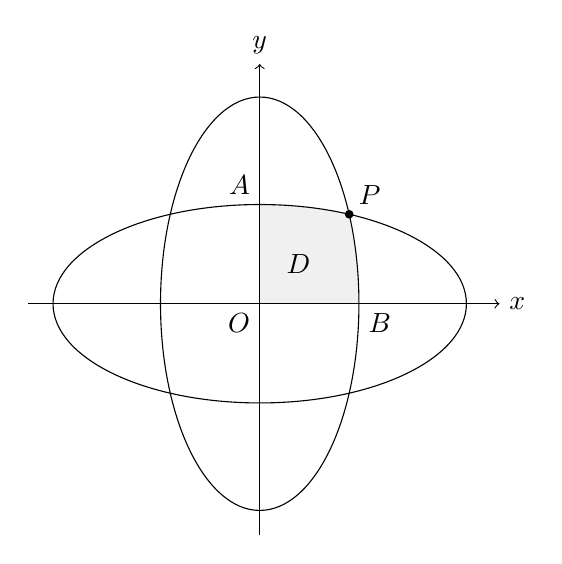
\begin{tikzpicture}[scale=1.05]
\fill[gray!12](0,0)--(1.2,0) arc[start angle=0,end angle=25.64,x radius=1.2,y radius=2.5] arc[start angle=64.36,end angle=90,x radius=2.5,y radius=1.2]--cycle;
\draw(0,0)ellipse(2.5 and 1.2);\draw(0,0)ellipse(1.2 and 2.5);
\draw[->](-2.8,0)--(2.9,0)node[right]{$x$};\draw[->](0,-2.8)--(0,2.9)node[above]{$y$};
\node[below left]at(0,0){$O$};\node[above left]at(0,1.2){$A$};\node[below right]at(1.2,0){$B$};\fill(1.082,1.082)circle(1.5pt)node[above right]{$P$};\node at(.47,.48){$D$};
\end{tikzpicture}\par{\small 图 5.2.5\quad 两椭圆的公共区域（重绘）}
\end{minipage}\end{center}

\entry{例 5.2.12}{含奇点的闭曲线积分（原解存疑）}{p.267}
求
\[
A=\oint_L\frac{x\dd y-y\dd x}{4x^2+y^2},
\]
其中 $L$ 是以 $(1,0)$ 为圆心、$R$ 为半径（$R\ne1$）的圆，取逆时针正向。
\par\textbf{原解（含疑点，见编校注）}\quad 记
\[
P=-\frac y{4x^2+y^2},\quad Q=\frac x{4x^2+y^2},\qquad
Q_x-P_y=\frac{y^2-4x^2}{(4x^2+y^2)^2},\quad (x,y)\ne(0,0).
\]
若 $R<1$，则 $L$ 不包原点，原书由 Green 公式得 $A=0$。

若 $R>1$，则 $L$ 包围原点。取其内部小椭圆
\[
L_1:\quad x=\frac\varepsilon2\cos\theta,\quad y=\varepsilon\sin\theta,\quad0\le\theta\le2\pi.
\]
原书在两曲线所围区域 $D$ 内用 Green 公式，得
\[
A=\oint_{L_1}\frac{x\dd y-y\dd x}{4x^2+y^2}.
\]
作代换，得到
\[
\int_0^{2\pi}\left(\frac12\cos^2\theta+\frac12\sin^2\theta\right)\dd\theta=\pi.
\]
所以原书结论为 $R>1$ 时 $A=\pi$。
\ednote{原书此步 Green 推断与所列旋度不符，题解待核。本稿保留原书所列导数与后续原结论。编校核算：由题面 $P,Q$ 直接求导，应有 $Q_x=P_y=(y^2-4x^2)/(4x^2+y^2)^2$，故原书所印非零表达式并非两者之差。疑点在原书旋度计算与书面论证不一致，不能仅凭此误印断言末答错误；本核算不是原书新增解法。}
\begin{center}\begin{minipage}{\linewidth}\centering
\begin{tikzpicture}[scale=1.15]
\draw[->](-1.5,0)--(3.2,0)node[right]{$x$};\draw[->](0,-2)--(0,2.1)node[above]{$y$};
\draw[thick](1,0)circle(1.7);\draw[thick,navy](0,0)ellipse(.18 and .36);
\fill(1,0)circle(1.4pt)node[below right]{$(1,0)$};\node[below left]at(0,0){$O$};\node[right]at(.18,.32){$L_1$};\node[right]at(2.2,1.2){$L$};\node at(.8,.8){$D$};
\end{tikzpicture}\par{\small 图 5.2.6\quad 外圆与小椭圆（$R>1$ 情形，重绘）}
\end{minipage}\end{center}

\entry{例 5.2.13}{Green 公式证明零边值唯一性}{pp.267—268}
设 $D$ 为 $Oxy$ 平面内有限条逐段光滑曲线围成的区域，$f$ 在 $D$ 上二阶连续，满足
\[
f_{xx}+f_{yy}=2af_x+2bf_y+cf,
\]
其中 $a,b,c$ 为常数，$c\ge0$。证明：若 $f$ 在 $\partial D$ 上恒为零，则在 $D$ 上恒为零。
\prooftext 设 $P=-f(f_y-bf)$、$Q=f(f_x-af)$，则 $P,Q$ 有一阶连续偏导数，且
\begin{align*}
Q_x-P_y&=f_x^2+f_y^2+f(f_{xx}+f_{yy}-2af_x-2bf_y)\\
&=f_x^2+f_y^2+cf^2.
\end{align*}
边界上 $f=0$，从而 $P=Q=0$。由 Green 公式，
\[
0=\oint_{\partial D}P\dd x+Q\dd y
=\iint_D(Q_x-P_y)\dd x\dd y
=\iint_D(f_x^2+f_y^2+cf^2)\dd x\dd y.
\]
因 $c\ge0$，故 $f_x=f_y=0$，$f$ 为常数；再由边界上为零，得 $f$ 在 $D$ 上恒为零。

\entry{例 5.2.14}{带指数系数的零边值问题}{pp.268—269}
设 $D$ 由光滑封闭曲线 $L$ 围成，$f$ 在 $D$ 上二阶连续，满足
\[
e^yf_{xx}+e^xf_{yy}=0,
\]
且在 $L$ 上 $f$ 恒为零。证明：

（1）存在一阶连续的 $P,Q$，满足 $Q_x-P_y=e^y(f_x)^2+e^x(f_y)^2$。

（2）$f$ 在 $D$ 上恒为零。
\prooftext （1）令 $P=-e^xff_y$、$Q=e^yff_x$，则
\begin{align*}
Q_x-P_y&=e^y[(f_x)^2+ff_{xx}]+e^x[(f_y)^2+ff_{yy}]\\
&=e^y(f_x)^2+e^x(f_y)^2+f(e^yf_{xx}+e^xf_{yy})\\
&=e^y(f_x)^2+e^x(f_y)^2.
\end{align*}
（2）因边界上 $P,Q$ 均为零，故 $\oint_LP\dd x+Q\dd y=0$。由 Green 公式，
\[
0=\iint_D[e^y(f_x)^2+e^x(f_y)^2]\dd x\dd y.
\]
被积函数非负，且积分为零，所以 $D$ 上 $f_x=f_y=0$。故 $f$ 为常数，进而恒为零。

\entry{例 5.2.15}{圆盘上函数积分的估计}{p.269}
设 $D:x^2+y^2\le a^2$，$a>0$；$f$ 在 $D$ 上有连续偏导数，边界上 $f=0$。证明
\[
\left|\iint_Df\dd x\dd y\right|\le\frac{\pi a^3}{3}\max_{(x,y)\in D}\sqrt{f_x^2+f_y^2}.
\]
\prooftext 取 $\partial D$ 逆时针方向。由 Green 公式，
\[
\oint_{\partial D}-yf\dd x+xf\dd y=\iint_D(2f+xf_x+yf_y)\dd x\dd y.
\]
左端为零，因此 $2\iint_Df\dd x\dd y=-\iint_D(xf_x+yf_y)\dd x\dd y$。
由 Cauchy 不等式，
\[
|xf_x+yf_y|\le\sqrt{x^2+y^2}\sqrt{f_x^2+f_y^2}.
\]
故
\begin{align*}
2\left|\iint_Df\dd x\dd y\right|
&\le\iint_D\sqrt{x^2+y^2}\sqrt{f_x^2+f_y^2}\dd x\dd y\\
&\le\max_D\sqrt{f_x^2+f_y^2}\iint_D\sqrt{x^2+y^2}\dd x\dd y\\
&=\frac{2\pi a^3}{3}\max_D\sqrt{f_x^2+f_y^2},
\end{align*}
即得所证。

\entry{例 5.2.16}{Poincaré 不等式}{p.270（上半页）}
设 $D$ 为简单光滑闭曲线 $L$ 围成的区域，$f$ 在 $\overline D$ 上有连续偏导数，且 $L$ 上 $f(x,y)=0$。证明
\[
\iint_Df^2(x,y)\dd x\dd y\le\max_D\{x^2+y^2\}\cdot\iint_D[(f_x)^2+(f_y)^2]\dd x\dd y.
\]
\prooftext 记 $M=\max_D\{x^2+y^2\}$。在例 5.2.15 的证明中用 $f^2$ 代替 $f$，得
\[
2\iint_Df^2\dd x\dd y=-\iint_D(2xff_x+2yff_y)\dd x\dd y.
\]
由 Cauchy 积分不等式，
\begin{align*}
\iint_Df^2\dd x\dd y
&\le\iint_D\sqrt{x^2+y^2}\,|f(x,y)|\sqrt{f_x^2+f_y^2}\dd x\dd y\\
&\le\sqrt M\iint_D|f(x,y)|\sqrt{f_x^2+f_y^2}\dd x\dd y\\
&\le\sqrt M\left(\iint_Df^2\dd x\dd y\right)^{1/2}
\left(\iint_D[f_x^2+f_y^2]\dd x\dd y\right)^{1/2},
\end{align*}
由此得证。
\ednote{原书 Cauchy 估计中 $f$ 处应取绝对值，此处补正。}
